\documentclass[a4paper,titlepage,UTF8]{ctexbook}

% 导言区
% 包
\usepackage{xeCJK} % 导入中文支持包
\usepackage[colorlinks, linkcolor=blue]{hyperref} % 超链接的颜色设置为红色
\usepackage{xcolor}
\usepackage{listings}
\usepackage{geometry}
\usepackage{fancyhdr}
\usepackage{cite}
\usepackage[super]{gbt7714} % 中文文献包
\usepackage{graphicx} % 导入图片包
\graphicspath{{img/game/},{img/install/},{img/screenfetch/}}
\usepackage{subfig}
\usepackage{tabularx}
\usepackage{chngpage}
\usepackage{array}
\usepackage{parskip}

\newfontfamily\consolas{Consolas}

% green
\definecolor{mygreen}{rgb}{0, 0.6, 0}

% 页边距
\geometry{left=2.5cm,right=2.5cm,top=2.0cm,bottom=2cm}

% 页眉页脚
\pagestyle{empty}

\lstset{
	basicstyle=\small\consolas,
	numberstyle= \tiny, 
	keywordstyle= \color{ blue!70},
	commentstyle=\color{mygreen},
	frame=shadowbox, 
	rulesepcolor= \color{ red!20!green!20!blue!20},
	columns=flexible, % 等宽字体
} 

% 中文设置
\setCJKmainfont{思源宋体}

% 英文设置
\setmainfont{JetBrains Mono}

% 标题页
\title{QtDocumentCN}
\CTEXoptions[today=small]
 % 标题左对齐
\CTEXsetup[format={\Large}]{section}

% 首行缩进两个字符
%\setlength{\parindent}{2em}

\begin{document}
% 正文区(文稿区)
% 页眉页脚
\pagestyle{fancy}
\lhead{
\includegraphics[scale=0.1]{./img/logo.png}}
\renewcommand{\headrulewidth}{0.4pt}

\maketitle
\tableofcontents
\thispagestyle{empty} % 目录页不显示页码
\chapter{贡献}
\begin{figure}[hbt!]
	\centering
	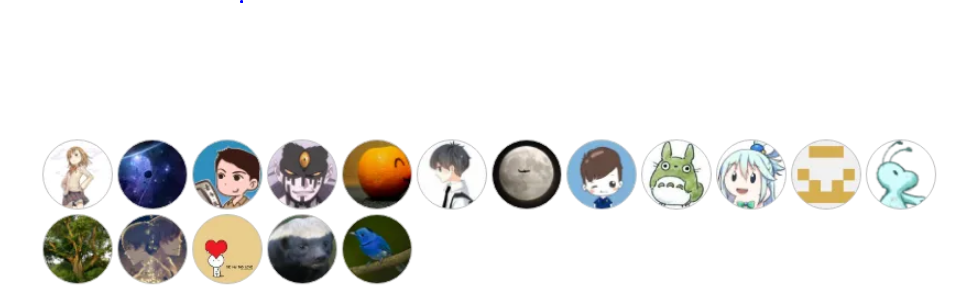
\includegraphics[width=\textwidth]{img/Contributors}
\end{figure}
\chapter{QSql}
QSql 命名空间

QSql 命名空间 里的 各种名样的标识符,已经被运用在 Qt SQL 各个模块中。\href{https://doc.qt.io/qt-5/qsql.html#details}{更多} 

\begin{tabular}{|c|c|p{1.5cm}|}
	\hline
	属性 & 方法 \\
	\hline
	头文件 & \#include <QSql>\\      
	\hline
	qmake & QT += sql\\      
	\hline
\end{tabular}

类型

\resizebox{\textwidth}{!}{ % Latex表格宽度超出文本宽度
\begin{tabular}{|c|l|}
	\hline
	 &  \\
	\hline
	enum & Location \{ BeforeFirstRow, AfterLastRow \}\\      
	\hline
	enum & NumericalPrecisionPolicy \{ LowPrecisionInt32, LowPrecisionInt64,LowPrecisionDouble,HighPrecision\}\\      
	\hline
	flags & ParamType \\
	\hline 
	enum & ParamTypeFlag \{ In, Out, InOut, Binary \} \\ 
	\hline
	enum & TableType \{ Tables, SystemTables, Views, AllTables \}\\
	\hline
\end{tabular}
}


细节的介绍 

查看 \href{https://doc.qt.io/qt-5/qtsql-index.html}{Qt SQL}

类型 文档

enum QSql::Location


此枚举类型描述特殊的sql导航位置


\begin{tabular}{|c|c|c|}
	\hline
	常量	& 值 & 介绍 \\
	\hline
	QSql::BeforeFirstRow&-1&在第一个记录之前\\
	\hline
	QSql::AfterLastRow&-2&在最后一个记录之后\\
	\hline
\end{tabular}

另请参阅 \href{https://doc.qt.io/qt-5/qsqlquery.html#at}{QSqlQuery::at()}

enum QSql::NumericalPrecisionPolicy


数据库中的数值可以比它们对应的C++类型更精确。此枚举列出在应用程序中表示此类值的策略。


\resizebox{\textwidth}{!}{ % Latex表格宽度超出文本宽度
\begin{tabular}{|c|c|c|}
	\hline
	常量	& 值 & 介绍 \\
	\hline
	QSql::LowPrecisionInt32	&0x01 &对于32位的整形数值。在浮点数的情况下,小数部分将会被舍去。\\
	\hline
	QSql::LowPrecisionInt64	&0x02 &对于64位的整形数值。在浮点数的情况下,小数部分将会被舍去。\\
	\hline
	QSql::LowPrecisionDouble&0x04 &强制双精度值。这个默认的规则\\
	\hline
	QSql::HighPrecision	&0&字符串将会维技精度\\
	\hline
\end{tabular}
}

注意: 如果特定的驱动发生溢出,这是一个真实行为。像 Oracle数据库在这种情形下,就会返回一个错误。


enum QSql::ParamTypeFlag


flags QSql::ParamType


这个枚举用于指定绑定参数的类型

\begin{tabular}{|l|l|l|}
	\hline
		常量	& 值 & 介绍 \\
	\hline
	QSql::In&0x00000001&这个参数被用于向数据库里写入数据\\
	\hline
	QSql::Out&0x00000002&这个参数被用于向数据库里获得数据\\
	\hline
	QSql::InOut&In | Out&这个参数被用于向数据库里写入数据;使用 查询 来向数据库里,重写数据\\
	\hline
	QSql::Binary&0x00000004&如果您想 显示数据为 原始的二进制数据,那么必须是 OR'd 和其他的标志一 起使用\\
	\hline
\end{tabular}

类型参数 类型定义为 \href{https://doc.qt.io/qt-5/qflags.html}{QFlags}. 它被存放在 一个 OR与 类型参数标志的值 的组合。






\chapter{QSqlDatabase}
QSqlDatabase 类 用于处理数据库的连接

\begin{tabular}{|c|c|p{1.5cm}|}
	\hline
	属性 & 方法 \\
	\hline
	头文件 & \#include <QSql>\\      
	\hline
	qmake & QT += sql\\      
	\hline
\end{tabular}\\

类型

\begin{tabular}{|c|c|}
	\hline
	&  \\
	\hline
	enum & Location \{ BeforeFirstRow, AfterLastRow \}\\      
	\hline
	enum & NumericalPrecisionPolicy \{ LowPrecisionInt32, LowPrecisionInt64,LowPrecisionDouble,HighPrecision\}\\      
	\hline
	flags & ParamType \\
	\hline 
	enum & ParamTypeFlag \{ In, Out, InOut, Binary \} \\ 
	\hline
	enum & TableType \{ Tables, SystemTables, Views, AllTables \}\\
	\hline
\end{tabular}\\

细节的介绍 \\

查看 \href{https://doc.qt.io/qt-5/qtsql-index.html}{Qt SQL}

类型 文档\\ 

enum QSql::Location


此枚举类型描述特殊的sql导航位置


\begin{tabular}{|c|c|c|}
	\hline
	常量	& 值 & 介绍 \\
	\hline
	QSql::BeforeFirstRow&-1&在第一个记录之前\\
	\hline
	QSql::AfterLastRow&-2&在最后一个记录之后\\
	\hline
\end{tabular}\\

另请参阅 \href{https://doc.qt.io/qt-5/qsqlquery.html#at}{QSqlQuery::at()}

enum QSql::NumericalPrecisionPolicy


数据库中的数值可以比它们对应的C++类型更精确。此枚举列出在应用程序中表示此类值的策略。


\begin{tabular}{|c|c|c|}
	\hline
	常量	& 值 & 介绍 \\
	\hline
	QSql::LowPrecisionInt32	&0x01 &对于32位的整形数值。在浮点数的情况下,小数部分将会被舍去。\\
	\hline
	QSql::LowPrecisionInt64	&0x02 &对于64位的整形数值。在浮点数的情况下,小数部分将会被舍去。\\
	\hline
	QSql::LowPrecisionDouble&0x04 &强制双精度值。这个默认的规则\\
	\hline
	QSql::HighPrecision	&0&字符串将会维技精度\\
	\hline
\end{tabular}\\

注意: 如果特定的驱动发生溢出,这是一个真实行为。像 Oracle数据库在这种情形下,就会返回一个错误。\\


enum QSql::ParamTypeFlag


flags QSql::ParamType


这个枚举用于指定绑定参数的类型

\begin{tabular}{|l|l|l|}
	\hline
	常量	& 值 & 介绍 \\
	\hline
	QSql::In&0x00000001&这个参数被用于向数据库里写入数据\\
	\hline
	QSql::Out&0x00000002&这个参数被用于向数据库里获得数据\\
	\hline
	QSql::InOut&In | Out&这个参数被用于向数据库里写入数据;使用 查询 来向数据库里,重写数据\\
	\hline
	QSql::Binary&0x00000004&如果您想 显示数据为 原始的二进制数据,那么必须是 OR'd 和其他的标志一 起使用\\
	\hline
\end{tabular}

类型参数 类型定义为 \href{https://doc.qt.io/qt-5/qflags.html}{QFlags}. 它被存放在 一个 OR与 类型参数标志的值 的组合。






\end{document}